\subsection{Pupa}
Para el análisis de la tasa de desarrollo, en días, de las pupas, del Aedes aegypti, incluyeron
las pupas que se desarrollaron completamente para pasar a ser un adulto. Existen diversos
estudios, que han reportado que tasa de desarrollo de las pupas, se encuentra influenciada por la
temperatura y varía de acuerdo a las localidades y subespecies. A continuación se mencionaran
algunos estudios realizados correspondientes a la tasa de desarrollo en días de la pupa, con el
fin de realizar una comparación con los resultados obtenidos mediante el proceso evolutivo.

En \cite{rueda1990temperature}, se reporta el efecto de temperaturas constantes sobre las tasas
de desarrollo, el crecimiento y la supervivencia de los estados inmaduros de Aedes aegypti,
determinadas en condiciones de laboratorio, y el modelo dependiente de la temperatura de
\cite{sharpe1977reaction}. En la \tabref{tab:desarrollo-pupa-rueda1990temperature-test} se
presentan los resultados obtenidos a seis temperaturas constantes(15-34 \textcelsius) en
comparación a los obtenidos en \cite{rueda1990temperature}.


\begin{table}[!htbp]
    \begin{minipage}{\textwidth}
    \centering
        \caption{ \label{tab:desarrollo-pupa-rueda1990temperature-test} Análisis de la tasa de desarrollo de las pupas del Aedes aegypti a 6 temperaturas constantes
        (15-34 \textcelsius).}
        \begin{tabular}{p{4cm} c c c c c c c}
            \hline\\
            Resultados & 15\textcelsius & 20\textcelsius & 25\textcelsius & 27\textcelsius
            & 30\textcelsius & 34\textcelsius &  Media General\\
            \hline
            \hline \\
            Media Observada$^{a}$   & 8,49 & 3,11 & 3,03 & 1,79 & 1,82 & 1,09 & 3,22\\
            Mediana Observada$^{a}$ & 8,46 & 3,04 & 2,98 & 1,81 & 1,79 & 1,05 & 3,19\\
            Media Predicha$^{b}$    & 6,9  & 4,1  & 2,5  & 2,06 & 1,56 & 1,08 & 3,03\\
            Media obtenida$^{c}$    & 6,14 & 4,26 & 2,17 & 2,17 & 1,11 & 1,14 & 2,83\\
        \end{tabular}
        \footnotetext[1]{Valores observados por \cite{rueda1990temperature}.}
        \footnotetext[2]{Resultados obtenidos por el modelo de \cite{sharpe1977reaction}.}
        \footnotetext[3]{Resultados obtenidos mediante el proceso evolutivo.}
    \end{minipage}
\end{table}

En la \figref{fig:desarrollo-pupa-rueda1990}, se puede observar una comparativa con los
valores observados en \cite{rueda1990temperature}, la media predicha y la media obtenida. En
general se obtuvo un desarrollo de $2,83$ días para 6 temperaturas contantes (15, 20, 25, 27,
30, 34 \textcelsius), con una diferencia de $0,39$ y $0,36$ días con la media general de los
valores observados en \cite{rueda1990temperature} para la media y la mediana observada respectivamente. En relación a la media predicha, que fue obtenida mediante el modelo de
\cite{sharpe1977reaction}, se obtuvo una diferencia de $0,2$ días con la media obtenida mediante el
proceso evolutivo.

\begin{figure}[!htbp]
    \centering
    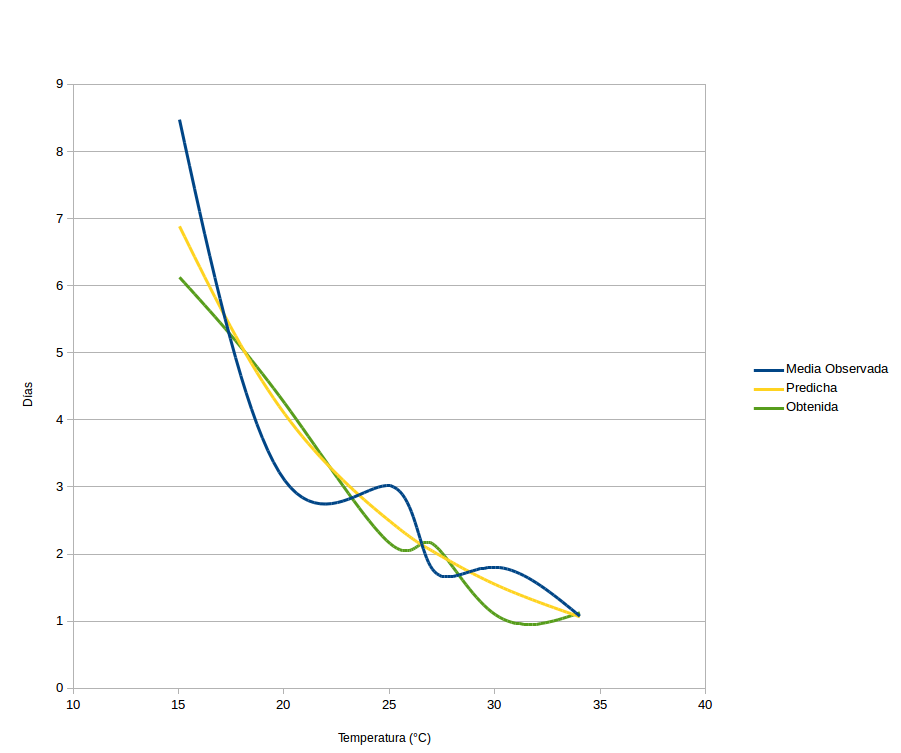
\includegraphics[width=1\textwidth]{capitulo-6/graphics/desarrollo-pupa-rueda.png}
    \caption{\label{fig:desarrollo-pupa-rueda1990}
    Comparativa entre ,la media obtenida, la media predicha y las media observada por \cite{
    rueda1990temperature} en distintas poblaciones a 6 temperaturas contantes (15-34 \textcelsius)
    para las tasas de desarrollo de las pupas del Aedes aegypti.}

\end{figure}


En \cite{BESERRA2006}, se presentan los requerimientos térmicos para el desarrollo del Aedes
aegypti en condiciones naturales, para 5 cepas de Aedes aegypti, provenientes de diferentes
poblaciones, a 5 temperaturas constantes (18-34\textcelsius). En la
\tabref{tab:desarrollo-pupa-baserra2006-test} se presentan los resultados obtenidos a cinco
temperaturas constantes(15-34 \textcelsius) en comparación a las tasas de desarrollo obtenidas en
\cite{BESERRA2006} para las pupas del Aedes aegypti.

\begin{table}[!htbp]
    \begin{minipage}{\textwidth}
        \caption{\label{tab:desarrollo-pupa-baserra2006-test} Análisis de la tasa de desarrollo de
        las pupas del Aedes aegypti a 5 temperaturas constantes (15-34 \textcelsius).}
        \begin{tabular}{p{4cm} c c c c c c }
            \hline\\
            Población    &18 \textcelsius & 22 \textcelsius & 26 \textcelsius & 30 \textcelsius
            & 34 \textcelsius & Media General\\
            \hline
            \hline \\
            Boqueirão$^{a}$      & 7,2  & 3,2  & 2,7  & 1,2  & 1,4  & 3,14\\
            B, dos Santos$^{a}$  & 6,4  & 3,2  & 2,1  & 2,1  & 1,2  & 3\\
            C, Grande$^{a}$      & 6,7  & 2,7  & 2,4  & 1,6  & 1,6  & 3\\
            Itaporanga$^{a}$     & 6,6  & 3,2  & 2,3  & 1,4  & 1,4  & 2,98\\
            Remígio$^{a}$        & 6,3  & 3,3  & 2,3  & 1,1  & 1,1  & 2,82\\
            Media obtenida$^{c}$ & 5,24 & 3,21 & 2,17 & 1,11 & 1,14 & 2,57\\
        \end{tabular}
        \footnotetext[1]{Los valores presentados para estas poblaciones fueron tomados de
         \cite{BESERRA2006}.}
        \footnotetext[2]{Resultados obtenidos mediante el proceso evolutivo.}
    \end{minipage}
\end{table}

En la \figref{fig:desarrollo-pupa-baserra2006}, se puede observar una comparativa con los
valores observados en \cite{BESERRA2006}, la media predicha y la media obtenida. En general se
obtuvo un desarrollo de $2,57$ días para 5 temperaturas contantes (18, 22, 26, 30, 34
\textcelsius), con una diferencia de $0,57$, $0,43$, $0,43$, $0,41$ y $0,25$ días con la media
general de los valores observados en \cite{BESERRA2006} para las poblaciones de Boqueirão, B. dos
Santos, C. Grande, Itaporanga y Remígio respectivamente. En relación a la media predicha, que fue
obtenida mediante el modelo de \cite{sharpe1977reaction}, se obtuvo una diferencia de $0,09$ días
con la media obtenida.


\begin{figure}[!htbp]
    \centering
    \begin{subfigure}[b]{0.45\textwidth}
            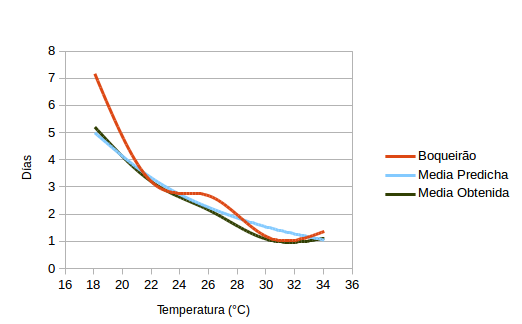
\includegraphics[width=\textwidth]{capitulo-6/graphics/desarrollo-pupa-1.png}
            \caption{Tasa de desarrollo de Boqueirão en comparación con la media predicha y obtenida.}
    \end{subfigure}
    ~~~~
    \begin{subfigure}[b]{0.45\textwidth}
            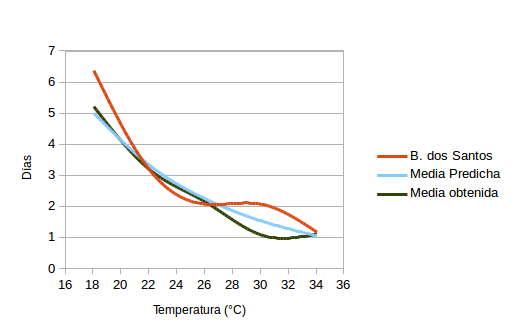
\includegraphics[width=\textwidth]{capitulo-6/graphics/desarrollo-pupa-2.png}
            \caption{Tasa de desarrollo de B. dos Santos en comparación con la media predicha y obtenida.}

    \end{subfigure}
    \begin{subfigure}[b]{0.45\textwidth}
            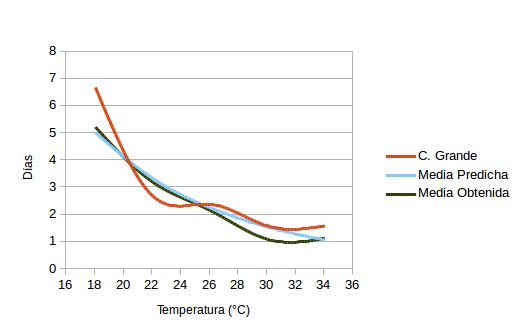
\includegraphics[width=\textwidth]{capitulo-6/graphics/desarrollo-pupa-3.png}
            \caption{Tasa de desarrollo de C. Grande en comparación con la media predicha y obtenida.}
    \end{subfigure}
    ~~~~
    \begin{subfigure}[b]{0.45\textwidth}
            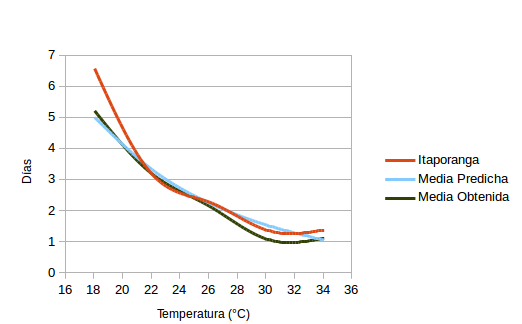
\includegraphics[width=\textwidth]{capitulo-6/graphics/desarrollo-pupa-4.png}
            \caption{Tasa de desarrollo de Itaporanga en comparación con la media predicha y obtenida.}

    \end{subfigure}
    \begin{subfigure}[t]{0.45\textwidth}
            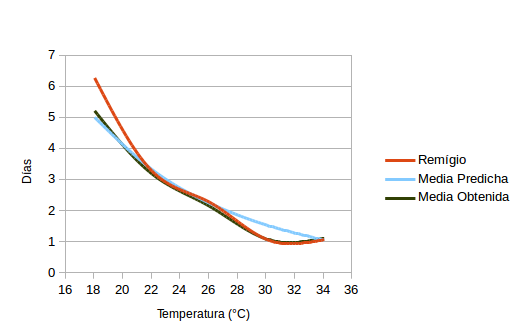
\includegraphics[width=\textwidth]{capitulo-6/graphics/desarrollo-pupa-5.png}
            \caption{Tasa de desarrollo de Remígio en comparación con la media predicha y obtenida.}
    \end{subfigure}
    ~~~~
    \begin{subfigure}[t]{0.45\textwidth}
            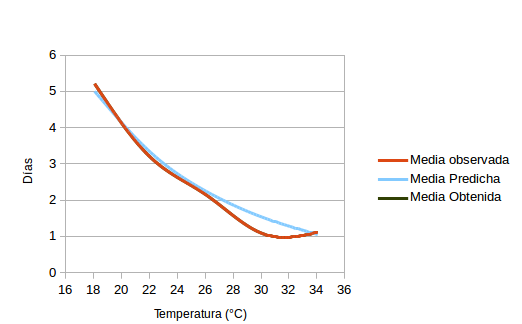
\includegraphics[width=\textwidth]{capitulo-6/graphics/desarrollo-pupa-6.png}
            \caption{Media observada en los poblados de Boqueirão, B. dos Santos, C. Grande, Itaporanga, Remígio en comparación con la media predicha y obtenida.}

    \end{subfigure}

    \caption{\label{fig:desarrollo-pupa-baserra2006}
    Comparativa entre ,la media obtenida, la media predicha y las medias observadas por \cite{
    BESERRA2006} en distintas poblaciones a 5 temperaturas contantes (18-34 \textcelsius) para
    las tasas de desarrollo de las pupas del Aedes aegypti.}

\end{figure}
